\section{Historical experiments and separate evidence cohorts}\label{app:historical-experiments}
\subsection{Datasets, references and evidence cohorts}
We evaluate fixed-center fidelity, actual proof cost and changing-center reuse separately. The capped native studies use Gaussian-easy/hard, a margin-synthetic corpus, MNIST, Fashion-MNIST, Gisette, Arcene and nonzero 20 Newsgroups TF--IDF. Table~\ref{tab:datasets-a} records their caps and the earlier fixed-center proof catalogs. Image and text sources are documented by their original dataset references \cite{lecun1998,fashion2017,gisette2004,arcene2004,news20data}.
\begin{table*}[tp]
\caption{Capped native corpora and actual fixed-center proof catalogs.}\label{tab:datasets-a}
\centering\small
\begin{adjustbox}{max width=\textwidth}
\begin{tabular}{@{}lrrrl@{}}
\toprule
Corpus & Native rows & Features $d$ & Audit rows/start & Proof catalog $N$ \\
\midrule
Gaussian-easy & 2,000 & 256 & 800 & -- \\
Gaussian-hard & 2,000 & 512 & 800 & 32 ($k=5,10$) \\
Margin-synthetic & 1,000 & 128 & 400 & -- \\
MNIST & 5,000 & 784 & 2,000 & 16; 64 ($k=5$) \\
Fashion-MNIST & 5,000 & 784 & 2,000 & 16 ($k=5$) \\
Gisette & 3,000 & 5,000 & 1,200 & 8 ($k=5$) \\
Arcene & 100 & 10,000 & 40 & -- \\
20 Newsgroups & 2,913 & 2,000 & 1,166 & 16 ($k=5$) \\
\bottomrule
\end{tabular}
\end{adjustbox}
\par\vspace{3pt}\begin{minipage}{0.98\textwidth}\footnotesize Each capped corpus uses a 60/40 fit/audit split and $k=5,10$ with three starts. Image subsets are sampled by the loader. Text starts with at most 3,000 training documents; zero vectors are removed, leaving 2,913. Gisette uses a 3,000-row cap; Arcene uses 100 cached training rows. Margin-synthetic is used here only for fixed-center and geometry tests, not a DBSCAN proof.\end{minipage}
\end{table*}


Historical new-center native studies add two neural representations: 2,048-dimensional ResNet-50 average-pool features for a seed-0 sample of 10,000 CIFAR-10 training images, and 384-dimensional \texttt{all-MiniLM-L6-v2} embeddings of nonempty 20 Newsgroups training documents \cite{krizhevsky2009cifar,he2016resnet,reimers2019sbert,minilmv2model}. The embedding builder records preprocessing and source-selection metadata; experiment loaders cap each embedding corpus at 5,000 rows. The historical changing-center proof workloads use 64 held-out records from MNIST and CIFAR embeddings, plus a 256-record MNIST scale check, at full feature dimensions. The completed review-control cohort adds 1,024 MNIST records. Those historical proof cohorts use $k=5$; the new paired study varies $k$ as specified below.

In the historical cohorts, training uses 60\% of the loaded corpus and auditing uses the remaining 40\%, after removing zero-norm rows. The deployed centers use $k$-means with five initializations and seed~0 in the proof workload. Both learned and PCA bases use the training split. Scaling uses the loaded corpus maximum; image source partitions are pooled by the original loader, and TF--IDF vocabulary fitting precedes the center/PCA split. These are fixed-corpus audits rather than unseen-data predictive-learning benchmarks. The stored embedding vectors are the inputs to the proof; the neural feature extractor is not proved.

Earlier capped fixed-center native results use three fitted starts. The completed follow-up uses five starts on all eight capped corpora, $k=5,10$, widths 16/32/64/128 where eligible, and ten random maps: 80 corpus/$k$/start cells and 9,900 raw rows across methods and widths. A separate full-cached image/text study uses five starts and the complete cached corpora, giving 28,000 audit rows per image corpus and 4,378 text audit rows per start. The new-center native study comprises 60 corpus/$k$/start jobs across ten corpora, $k=5,10$ and three starts, with one deployed-center control and twelve new scenarios per job. Its 227,604 raw method/map/scenario rows are correlated repetitions. Random maps are averaged within a cell before aggregate comparisons; eligible ranks differ by experiment.

\subsection{Proof implementation and timing policy}\label{app:historical-implementation}
The Go implementation uses gnark v0.16.3, gnark-crypto v0.21.0, Groth16 over BN254, Poseidon2 row-Merkle commitments, batched range checks and bounded comparisons. Main proof measurements run on one Linux host with four logical CPUs and approximately 7.8\,GiB RAM; a separate same-input Windows portability check is reported below. The reuse queue sets \texttt{GOMAXPROCS}=4 and \texttt{OMP\_NUM\_THREADS}=4. Historical $N=64$ phases use one warmup where specified and three timed proof repetitions; the historical $N=256$ scale check uses one timed repetition per sample. The completed review-control cohort uses one measured repetition per sample and one initial warmup. We add each sample's median proving time to its measured witness time. The process guard limits constraint count to 1.6 million per circuit. The five-start native follow-up runs three worker groups with one OpenMP/BLAS thread each.

For the historical workloads and the first $L$ center sets, cumulative cost adds native Go preparation, compilation, setup and witness/proving costs actually recorded for that method. Reuse methods pay Stage~1 and one query setup once. The evaluated cached/affine methods pay their center-specific preparation, Stage~1 and setup for every set. Historical Full has no Stage~1; its center-specific setup is charged for every set. Its catalog proving component is extrapolated by multiplying one measured batch by $N/b_{\rm Full}$, where the resource guard selects batch eight for MNIST and two for CIFAR embeddings. Each Full batch is proved and verified, but its whole-catalog total is not a measured full run. The other methods prove all catalog rows and requested batches. These historical totals exclude verification, fitting, warmups, I/O and public new-center-statistic preparation. The new public-center Full controls instead reuse setup and prove complete catalogs; Section~\ref{sec:review-controls} distinguishes those measurements and normalizes native answer-construction costs.

Every generated proof is checked during the proving run. The snapshot analysis checks phase completeness, recorded verification counts, positive timings and exact reconstruction of exported witness/proving sums from saved samples. It validates 1,092 captured file hashes and matching copies of the five available Python sources. Each $N=64$ cohort records 1,532 verified proof samples; the $N=256$ cohort records 6,098. These counts describe the recorded verifier checks, not a fresh independent replay of every saved reuse proof. The binary hash is retained; Go source was not present in the remote runtime directory. AI-assisted development was used for experiment and analysis code and for manuscript preparation; the source package records the numerical exports and the checks applied to them.

\subsection{Metrics}
Assignment agreement and adjusted Rand index (ARI) compare method assignments with nearest original-space centers, not class labels. Fixed-center tables explicitly distinguish quantized Full from floating Full. For new centers, agreement uses floating Full on the same held-out records. Cost error is
\begin{equation}
e_\Psi=\frac{\widehat\Psi/(T^4S^2)}{\Phi_I(\mathcal C')}-1
\end{equation}
for head/energy methods, with divisor $S^2$ for cached/affine/Full. Mean absolute cost error is the mean of $|e_\Psi|$ across the specified center sets or matched native cells. It includes both assignment and distance-estimation effects. Means in the proof workload exclude the deployed set, leaving nine new sets; the timing workload includes all ten. Repeated timing samples do not supply independent geometric trials or confidence intervals over future models.



\subsection{Earlier complete-catalog controls: a separate evidence cohort}
The following completed 14-case cohort uses different fitted centers and timing boundaries from the paired study. Its actual 1,024-record proofs establish scale for absolute certificates, rather than completion of the new paired scale cases.

\subsection{Completed matched controls and actual catalog scaling}\label{sec:review-controls}
The completed review-control campaign comprises four exact public-center Full cases and ten plain/certified reuse cases. It audits MNIST catalogs of 64, 256 and 1,024 records and a 64-record CIFAR/ResNet catalog, each against ten approved public center sets. Learned/energy and PCA/energy use the same original integer rows, center sets, catalog root and task coverage as their exact control. The original rank-15 configurations use $T=4096$ and batch 64. Two predeclared MNIST $N=256$ pilots use rank 63, $T=16384$ and batch 16. All cases finish; no table infers proof completion from native execution or extrapolates unproved catalog batches.

Exact Full takes the full center coordinates as public inputs, authenticates original rows directly, and pays one compilation/setup for all ten sets. It needs no Stage~1. Under the common 1.6-million-constraint guard, Full uses batch eight for MNIST and two for CIFAR. Its four controls contain 80, 320, 1,280 and 320 actual proofs respectively. Every proof passes independent public-only replay, and local integer-reference analysis reproduces every saved Full label and aggregate cost (Table~\ref{tab:public-full-complete}). Different feasible batches are part of the measured resource-bounded configurations, rather than a claim that one batch is universally optimal.
\begin{table*}[tp]
\caption{Completed exact public-center Full controls. One setup serves all ten center sets; every catalog batch is proved and independently replayed. Peak RSS describes the prover process tree, excluding the Python driver. Component costs include native answer construction.}\label{tab:public-full-complete}
\centering\small
\begin{adjustbox}{max width=\textwidth}
\begin{tabular}{@{}llllll@{}}
\toprule
Catalog & Batch & Proofs & Constraints & Cost (s) & Peak RSS (GiB) \\
\midrule
CIFAR/ResNet $N=64$ & 2 & 320 & 1,061,820 & 5,351.1 & 2.19 \\
MNIST $N=64$ & 8 & 80 & 1,416,899 & 1,715.9 & 3.19 \\
MNIST $N=256$ & 8 & 320 & 1,422,913 & 6,237.9 & 3.21 \\
MNIST $N=1024$ & 8 & 1280 & 1,428,927 & 24,681.3 & 3.27 \\
\bottomrule
\end{tabular}
\end{adjustbox}
\end{table*}


For each deployment alternative, component cost includes native preparation, Stage~1 where applicable, query compilation/setup, native answer construction, witnesses and measured proving. Shared preprocessing is charged once; the exploratory plain-query phase is not charged to the certified alternative. Verification, warmups, fitting, I/O and public-center-statistic preparation are excluded and retained separately in the raw phase records. The first frozen Full worker omitted native answer construction from its CSV; we reconstruct that component from its saved samples without changing original results. All cases run serially on the same host, with one measured repetition per sample and one initial warmup. These totals measure a chosen deployment's components, not end-to-end online latency or timing variability across machines.

At $N=1024$, exact Full costs 24,681.3\,s, compared with 4,778.1\,s for plain learned reuse and 4,861.0\,s for certified learned reuse. The Full/component-cost ratios are 5.17 and 5.08. Main learned certified ratios range from 4.15 on MNIST $N=64$ to 8.07 on CIFAR $N=64$ (Table~\ref{tab:matched-public-full}). PCA/energy costs are similar: its $N=1024$ plain and certified totals are 4,823.8 and 4,904.6\,s. There is no general proof-speed advantage from selecting the learned basis instead of PCA at this representation width.
\begin{table*}[tp]
\caption{Completed matched audits over ten public center sets, rank 15 and $T=4096$. Each alternative pays preparation and setup once; every catalog row is proved. Component costs include native answer construction and exclude verification, fitting, warmups, I/O and public-center preparation. Full/certified compares different fidelity guarantees.}\label{tab:matched-public-full}
\centering\small
\begin{adjustbox}{max width=\textwidth}
\begin{tabular}{@{}lllllll@{}}
\toprule
Catalog & Method & Exact Full (s) & Plain (s) & Certified (s) & Full / certified & Cert. overhead (\%) \\
\midrule
CIFAR/ResNet $N=64$ & Learned + energy & 5,351.1 & 639.7 & 663.2 & 8.07 & 3.67 \\
CIFAR/ResNet $N=64$ & PCA + energy & 5,351.1 & 629.8 & 646.6 & 8.28 & 2.66 \\
MNIST $N=64$ & Learned + energy & 1,715.9 & 361.9 & 413.5 & 4.15 & 14.26 \\
MNIST $N=64$ & PCA + energy & 1,715.9 & 367.3 & 419.9 & 4.09 & 14.33 \\
MNIST $N=256$ & Learned + energy & 6,237.9 & 1,274.3 & 1,309.2 & 4.76 & 2.74 \\
MNIST $N=256$ & PCA + energy & 6,237.9 & 1,271.1 & 1,309.7 & 4.76 & 3.04 \\
MNIST $N=1024$ & Learned + energy & 24,681.3 & 4,778.1 & 4,861.0 & 5.08 & 1.74 \\
MNIST $N=1024$ & PCA + energy & 24,681.3 & 4,823.8 & 4,904.6 & 5.03 & 1.68 \\
\bottomrule
\end{tabular}
\end{adjustbox}
\end{table*}


The 1,024-record learned case replays 1,344 proofs: 1,024 Stage~1 proofs, 160 plain queries and 160 certified queries. Adding certification increases its query constraints from 616,148 to 740,617, but raises total component cost by only 1.74\% because preprocessing is shared. The corresponding PCA overhead is 1.68\%; at $N=64$, learned and PCA overheads are 14.26\% and 14.33\%. The largest exact Full process-tree RSS is 3.27\,GiB, versus 1.65\,GiB for the 1,024-record learned case; neither figure includes the Python driver or represents whole-host memory. Figure~\ref{fig:matched-scale} shows the measured scale result together with the difference between observed and certified accuracy.
\begin{figure*}[tp]
\centering
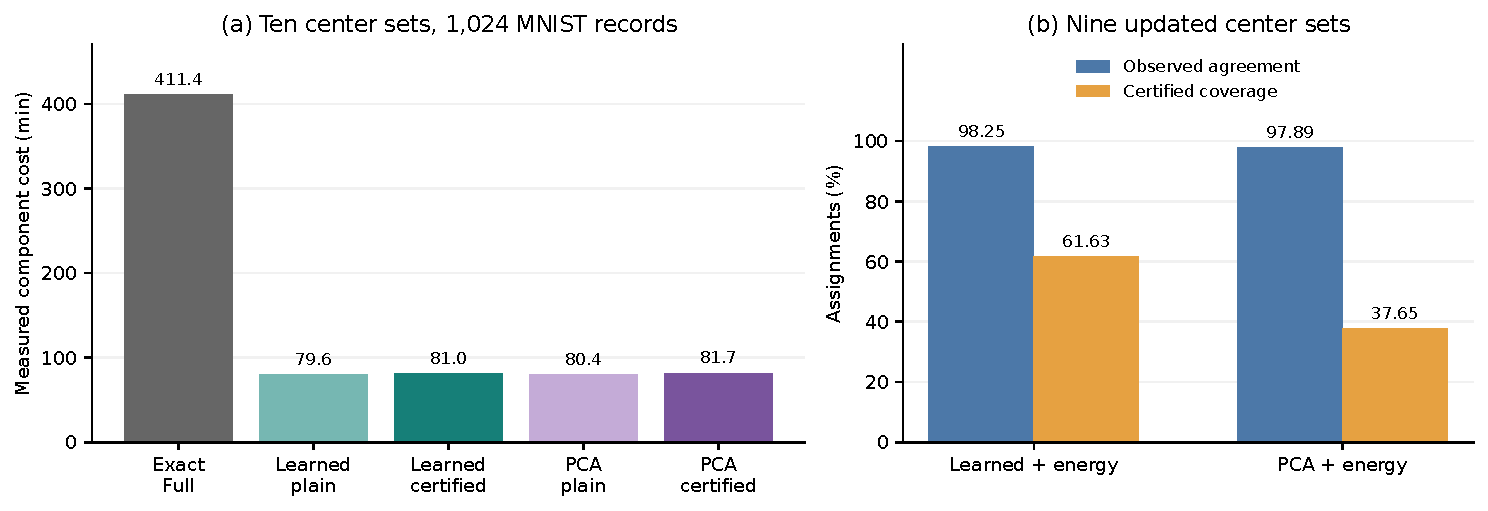
\includegraphics[width=\textwidth]{paper_results/review_controls/generated_completed_20261020/matched_scale.pdf}
\caption{Completed 1,024-record MNIST audit. (a) Measured component costs across ten public center sets, with setup and preprocessing charged once per alternative. Exact Full and approximate reuse provide different fidelity guarantees. (b) Mean agreement with quantized Full and guaranteed assignment coverage across nine updated sets. High empirical agreement does not imply that every assignment is certified.}
\label{fig:matched-scale}
\end{figure*}

\subsection{Proved accuracy envelopes and representation budgets}
The cost reductions come with a different verification contract. At $N=1024$, learned/energy agrees with quantized Full on 98.25\% of assignments on average across updated sets, while the proved correct-assignment count covers 61.63\% of rows on average and falls to 21.09\% for the worst update. Mean relative cost-interval width is 20.65\%. PCA gives 97.89\% agreement, 37.65\% coverage and 37.97\% width. Table~\ref{tab:matched-certificate-quality} reports all four main catalogs. Certified coverage is a lower bound for each individual set; an average across sets is descriptive and cannot replace its particular certificate.
\begin{table*}[tp]
\caption{Completed integer certificate quality at rank 15, $T=4096$. Agreement, certified coverage and relative cost-interval width are means across nine updated center sets. All checked intervals contain the exact quantized optimum; no certified assignment is incorrect.}\label{tab:matched-certificate-quality}
\centering\small
\begin{adjustbox}{max width=\textwidth}
\begin{tabular}{@{}llrrr@{}}
\toprule
Catalog & Method & Agreement (\%) & Certified (\%) & Width (\%) \\
\midrule
CIFAR/ResNet $N=64$ & Learned + energy & 99.48 & 60.76 & 24.00 \\
CIFAR/ResNet $N=64$ & PCA + energy & 98.44 & 39.76 & 33.58 \\
MNIST $N=1024$ & Learned + energy & 98.25 & 61.63 & 20.65 \\
MNIST $N=1024$ & PCA + energy & 97.89 & 37.65 & 37.97 \\
MNIST $N=256$ & Learned + energy & 98.31 & 59.20 & 20.51 \\
MNIST $N=256$ & PCA + energy & 97.44 & 35.98 & 38.10 \\
MNIST $N=64$ & Learned + energy & 98.26 & 52.26 & 20.80 \\
MNIST $N=64$ & PCA + energy & 96.53 & 30.03 & 38.19 \\
\bottomrule
\end{tabular}
\end{adjustbox}
\end{table*}


All 100 proved method/set outputs match the independent Python integer certificate, including assignment flags, count and both cost endpoints. Across 33,280 record/set evaluations, no certified assignment is incorrect and no interval misses the exact quantized optimum. These finite checks test implementation consistency; Proposition~\ref{prop:integer-envelope} supplies the general bound. The reported certified fractions and interval widths describe the guarantee available for each task without assigning a universal pass/fail threshold. The measured cost ratios do not establish equally exact services or authorize using small empirical point errors in place of the certificate.

The completed higher-rank proof pilots improve accuracy and certificate utility at increased component cost (Table~\ref{tab:proved-certificate-budget}). On MNIST $N=256$, learned rank-63/$T=16384$ gives 99.74\% agreement, 85.20\% certified coverage and 7.26\% mean width. Plain and certified totals are 1,731.2 and 1,834.8\,s, versus 1,274.3 and 1,309.2\,s at rank 15. PCA's higher-rank counterpart gives 99.70\% agreement, 80.51\% coverage and 8.88\% width. Both pilots replay all 576 proofs per case, including Stage~1. Rank, basis precision and query batch change together; these are combined configuration effects rather than an isolated causal effect of rank.
\begin{table*}[tp]
\caption{Completed predeclared MNIST $N=256$ rank-63, $T=16384$ proof pilots (batch 16). Quality means exclude the deployed set; costs cover all ten sets. Rank, precision and batching change together, so cost differences are configuration effects rather than an isolated rank ablation.}\label{tab:proved-certificate-budget}
\centering\small
\begin{adjustbox}{max width=\textwidth}
\begin{tabular}{@{}lllllll@{}}
\toprule
Method & Plain (s) & Certified (s) & Full / certified & Agreement (\%) & Certified (\%) & Width (\%) \\
\midrule
Learned + energy & 1,731.2 & 1,834.8 & 3.40 & 99.74 & 85.20 & 7.26 \\
PCA + energy & 1,753.5 & 1,850.1 & 3.37 & 99.70 & 80.51 & 8.88 \\
\bottomrule
\end{tabular}
\end{adjustbox}
\end{table*}


The native controls are retained separately in the artifact. The 1,024-record catalog extends the same held-out MNIST ordering; its first 256 quantized rows exactly match the earlier catalog. The deployed basis, scales, salts and ten center sets are retained without fitting on added audit rows. The original native preflight contains 80 method/set cells and 28,160 record/set evaluations; its rank-15 cases overlap the subsequently proved controls and are not independent observations.

A training-only native budget grid evaluates ranks 15/31/63/127 and basis scales 4096/16384 on the same 1,024 rows and ten sets. All cells are retained, and the rank-63 high-scale proof pilots were specified before inspecting these outcomes. Rank 15's high-scale control rescales the original rounded basis; larger ranks fit training data and round at each scale. At rank 63 and $T=16384$, learned/energy obtains 99.75\% agreement, 85.84\% mean coverage and 7.37\% width; rank 127 gives 90.32\% coverage and 4.64\% width. PCA also improves (Table~\ref{tab:native-certificate-budget}). These higher-rank 1,024-record cells are native calculations, not proof benchmarks; only the 256-record rank-63 configurations above have measured proof costs.
\begin{table*}[tp]
\caption{Native MNIST $N=1024$ budget controls (nine updated sets, quantized Full reference). All ranks and both basis scales are retained in the CSV artifact; this table shows the original configuration and larger-rank high-scale controls. These are not proof benchmarks.}\label{tab:native-certificate-budget}
\centering\small
\begin{adjustbox}{max width=\textwidth}
\begin{tabular}{@{}llrrrr@{}}
\toprule
Head rank / $T$ & Method & Agreement (\%) & Certified (\%) & Worst (\%) & Width (\%) \\
\midrule
15/4096 & Learned + energy & 98.25 & 61.63 & 21.09 & 20.65 \\
15/4096 & PCA + energy & 97.89 & 37.65 & 16.02 & 37.97 \\
31/16384 & Learned + energy & 99.36 & 76.86 & 31.05 & 12.28 \\
31/16384 & PCA + energy & 99.35 & 63.43 & 29.00 & 18.53 \\
63/16384 & Learned + energy & 99.75 & 85.84 & 45.80 & 7.37 \\
63/16384 & PCA + energy & 99.71 & 81.89 & 44.92 & 8.98 \\
127/16384 & Learned + energy & 99.86 & 90.32 & 59.86 & 4.64 \\
127/16384 & PCA + energy & 99.84 & 88.61 & 60.06 & 5.22 \\
\bottomrule
\end{tabular}
\end{adjustbox}
\end{table*}


Across the complete campaign, all 6,848 proofs pass independent public-only replay: 2,000 exact Full proofs and 4,848 Stage~1/plain/certified reuse proofs. Local analysis validates 208 captured metadata hashes, approved task coverage, matching original rows and centers, exact integer Full outputs and the independent certificate outputs. Targeted tests additionally reject altered roots, keys, indices, assignments and valid-range changes to certificate outputs. Optional tolerance-checker tests apply different user requirements to the same valid smoke certificate, separately from proof verification. The measurements themselves are reported as certified counts, cost intervals and observed agreement; application-specific tolerances are not treated as a benchmark success criterion.


\subsection{Fixed-center fidelity and the cached baseline}\label{sec:results}
On the full-cached five-start study, head+energy has mean ARI 0.999647 and agreement 99.9845\% against quantized Full, compared with PCA-16's 0.933384 and 97.2146\%. Against floating Full, head+energy agreement is 99.9108\%, while quantized Full itself reaches 99.9129\%. This separates input rounding from the additional basis-rounding effect. Table~\ref{tab:full-accuracy} gives the corpus/$k$ values; the capped eight-corpus results appear in \ref{app:fixed}.
\begin{table*}[tp]
\caption{Native fidelity on all cached image rows and nonzero cached text-training rows.}\label{tab:full-accuracy}
\centering\small
\begin{adjustbox}{max width=\textwidth}
\begin{tabular}{@{}lrrrrrr@{}}
\toprule
Corpus & $k$ & PCA ARI$_Q$ & Ours ARI$_Q$ & PCA agree.$_Q$ (\%) & Ours agree.$_Q$ (\%) & Ours agree.$_F$ (\%) \\
\midrule
MNIST & 5 & 0.97712 & 0.99974 & 99.072 & 99.990 & 99.989 \\
MNIST & 10 & 0.93466 & 0.99975 & 96.956 & 99.989 & 99.989 \\
Fashion-MNIST & 5 & 0.99601 & 0.99987 & 99.831 & 99.994 & 99.995 \\
Fashion-MNIST & 10 & 0.98809 & 0.99988 & 99.416 & 99.994 & 99.994 \\
20 Newsgroups & 5 & 0.88163 & 0.99920 & 95.724 & 99.968 & 99.712 \\
20 Newsgroups & 10 & 0.82280 & 0.99945 & 92.289 & 99.973 & 99.785 \\
\bottomrule
\end{tabular}
\end{adjustbox}
\par\vspace{3pt}\begin{minipage}{0.98\textwidth}\footnotesize Subscripts $Q$ and $F$ denote quantized-Full and floating-Full references. Five fitted starts per corpus/$k$; 60/40 fitting/audit split. MNIST and Fashion-MNIST: 70,000 rows each (28,000 audit rows). Text: 10,944 nonzero training documents, 2,000 TF--IDF features (4,378 audit rows). These are native runs, not whole-corpus proofs. Ours denotes both head/energy variants.\end{minipage}
\end{table*}


The earlier Poseidon2 fixed-center proof cohort provides the relevant control. For one whole-catalog MNIST query with $N=64$, head+energy+JL requires 306,274 constraints and 5.09\,s of proving, PCA-16 requires 472,429 and 6.30\,s, and cached exact answers require 197,147 and 3.44\,s. Its matched no-tail head+energy control has the same answers; the optional tail is unused by the fixed-center query. Including preprocessing in four distinct 32-row subset queries gives 268.38\,s for head+energy+JL versus 279.12\,s for PCA and 246.66\,s for cached answers (\ref{app:fixed}). Thus the single-set evidence favors the exact cached baseline, motivating the changing-center workload.

The completed five-start capped follow-up independently checks fixed-center numerical fidelity (Table~\ref{tab:fixed-five-starts}). At total width 16, the protected head with a JL residual tail has 100\% mean assignment agreement in floating arithmetic and 99.987\% after input/basis rounding, versus 95.340\% for plain PCA and 62.409\% for sparse JL. Its integer mean absolute cost error is 3.114\%, because this control estimates residual cost with a random tail. It is not the head+energy representation used by the main reuse circuit, and plain PCA here is not the stronger PCA+energy baseline. These native results support fixed-center fidelity rather than an additional proof-speed claim.
\begin{table*}[tp]
\caption{Five-start fixed-center fidelity at total width 16 on the capped eight-corpus campaign.}\label{tab:fixed-five-starts}
\centering\small
\begin{adjustbox}{max width=\textwidth}
\begin{tabular}{@{}lrrrrr@{}}
\toprule
Corpus & Head/JL float (\%) & Head/JL int. (\%) & PCA (\%) & Sparse JL (\%) & Int. $|e_\Psi|$ (\%) \\
\midrule
Gaussian-easy & 100.000 & 100.000 & 100.000 & 89.240 & 2.977 \\
Gaussian-hard & 100.000 & 100.000 & 98.600 & 45.235 & 1.297 \\
Margin synthetic & 100.000 & 99.975 & 82.950 & 60.350 & 2.833 \\
MNIST & 100.000 & 99.990 & 97.850 & 66.036 & 4.431 \\
Fashion-MNIST & 100.000 & 100.000 & 99.600 & 82.540 & 3.610 \\
Gisette & 100.000 & 99.967 & 97.767 & 45.371 & 1.718 \\
Arcene & 100.000 & 100.000 & 99.000 & 86.775 & 7.116 \\
20 Newsgroups & 100.000 & 99.966 & 86.955 & 23.726 & 0.927 \\
Mean & 100.000 & 99.987 & 95.340 & 62.409 & 3.114 \\
\bottomrule
\end{tabular}
\end{adjustbox}
\par\smallskip\begin{minipage}{0.98\textwidth}\footnotesize Assignment agreement is against floating original-space Full. There are 80 corpus/$k$/start cells (eight corpora, $k=5,10$, five starts); ten random maps are averaged within each cell. Head/JL preserves the deployed-center head and uses a sparse residual tail, not the energy statistic of the main reuse method. PCA here is plain PCA, not PCA with energy. The final column is mean absolute cost error of the integer Head/JL method. These native runs do not measure proof performance.\end{minipage}
\end{table*}


\subsection{Historical changing-center reuse: cumulative proof cost}
The workload audits the same catalog against ten center sets in this fixed order: the deployed set, two independent refits, two half-training subsample refits, Lloyd iterates 1/3/10 from another initialization, and perturbations of size 0.1/0.3 of median deployed-center spacing. These scenarios retain $k=5$. They use training data and do not form an optimization loop driven by private audit outputs. All methods receive the same integer catalog and quantized center sets.

Table~\ref{tab:reuse-cost} and Fig.~\ref{fig:reuse-cost} show the historical amortization comparison. For MNIST $N=64$, learned head+energy costs 311.4\,s at one set, 317.7\,s at two and 368.8\,s at ten. The center-specific cached baseline costs 250.1, 502.2 and 2,540.9\,s, respectively. For CIFAR embeddings, the ten-set totals are 635.2\,s versus 4,928.8\,s. The $N=256$ MNIST check gives 941.2, 977.4 and 1,267.6\,s for learned head+energy, versus 860.9, 1,724.8 and 8,642.8\,s for cached. The learned method crosses cached at $L=2$ in all three workloads; ten-set ratios are 6.89, 7.76 and 6.82. PCA+energy has essentially the same reuse cost: 366.2, 635.6 and 1,265.0\,s at ten sets. The result is amortization across changing centers, not faster individual query proofs than cached answers.
\begin{table*}[tp]
\caption{Cumulative cost across successive center sets, query batch $b=64$, $k=5$ (seconds).}\label{tab:reuse-cost}
\centering\small
\begin{adjustbox}{max width=\textwidth}
\begin{tabular}{@{}llrrr@{}}
\toprule
Catalog & Method & $L=1$ & $L=2$ & $L=10$ \\
\midrule
MNIST ($N=64$) & Cached exact & 250.1 & 502.2 & 2,540.9 \\
MNIST ($N=64$) & Exact affine & 277.9 & 552.0 & 2,758.4 \\
MNIST ($N=64$) & Full (extrapolated) & 342.3 & 684.6 & 3,473.6 \\
MNIST ($N=64$) & Span + energy & 282.3 & 287.4 & 329.1 \\
MNIST ($N=64$) & PCA + energy & 309.5 & 315.9 & 366.2 \\
MNIST ($N=64$) & Learned head + energy & 311.4 & 317.7 & 368.8 \\
CIFAR/ResNet-50 ($N=64$) & Cached exact & 490.3 & 980.3 & 4,928.8 \\
CIFAR/ResNet-50 ($N=64$) & Exact affine & 517.4 & 1,029.7 & 5,099.5 \\
CIFAR/ResNet-50 ($N=64$) & Full (extrapolated) & 493.6 & 984.2 & 4,781.0 \\
CIFAR/ResNet-50 ($N=64$) & Span + energy & 515.6 & 520.9 & 563.2 \\
CIFAR/ResNet-50 ($N=64$) & PCA + energy & 555.3 & 563.7 & 635.6 \\
CIFAR/ResNet-50 ($N=64$) & Learned head + energy & 554.9 & 563.7 & 635.2 \\
MNIST ($N=256$) & Cached exact & 860.9 & 1,724.8 & 8,642.8 \\
MNIST ($N=256$) & Exact affine & 889.4 & 1,777.1 & 8,851.4 \\
MNIST ($N=256$) & Full (extrapolated) & 808.9 & 1,574.4 & 8,036.5 \\
MNIST ($N=256$) & Span + energy & 904.2 & 926.4 & 1,105.6 \\
MNIST ($N=256$) & PCA + energy & 940.5 & 977.1 & 1,265.0 \\
MNIST ($N=256$) & Learned head + energy & 941.2 & 977.4 & 1,267.6 \\
\bottomrule
\end{tabular}
\end{adjustbox}
\par\smallskip\begin{minipage}{0.98\textwidth}\footnotesize Totals add measured native preparation, compilation, setup, witness generation and median proving times. All compressed/cached/affine catalog proofs were generated; Full catalog proving is extrapolated from one measured batch per set. The deployed set is first. Verification, fitting, warmups, I/O and public new-center preparation are excluded.\end{minipage}
\end{table*}

\begin{figure*}[tp]
\centering
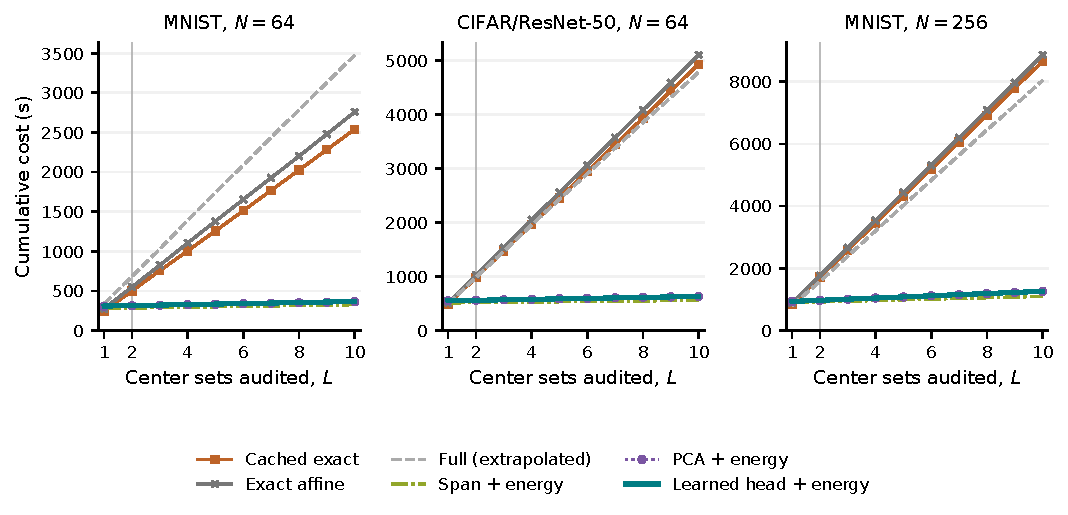
\includegraphics[width=\textwidth]{paper_results/reuse_revision/generated_20261020/cumulative_cost.pdf}
\caption{Historical cumulative cost for three completed changing-center workloads. The comparator Full embeds centers; this figure does not evaluate public-center Full. Learned head and PCA with energy almost overlap; savings over the tested center-specific cached/affine baselines come from reusing preprocessing and setup. The vertical line marks the second center set. Full catalog proving is extrapolated from one measured batch per set.}
\label{fig:reuse-cost}
\end{figure*}

For MNIST $N=64$, learned and PCA with energy have the same 519,896-constraint reuse circuit, compared with 343,455 for the narrower span-only head. Their Stage~1 circuits have 171,586 and 171,582 constraints per row. At $N=256$, the larger Merkle depth increases the shared reuse circuit to 568,022 constraints; learned Stage~1 uses 173,086 per row. For CIFAR, learned/PCA reuse requires 524,336 constraints and Stage~1 requires 432,049 per row. Selecting a different basis can therefore change accuracy without materially changing proof cost. Saved peak process-tree RSS is about 1.1--1.6\,GB for the 16-statistic methods; it excludes the Python driver and is not whole-pipeline memory.

\subsection{Changing-center fidelity}
The learned head has higher new-center agreement than PCA with energy on all three proof workloads: 98.26\% versus 96.53\% on MNIST $N=64$, 99.48\% versus 98.44\% on CIFAR embeddings, and 98.31\% versus 97.44\% on MNIST $N=256$ (Table~\ref{tab:reuse-quality}). The narrower deployed span alone reaches 83.51\%, 96.35\% and 85.76\%. Learned mean absolute cost errors are 0.228\%, 0.338\% and 0.178\%, compared with PCA/energy's 1.536\%, 0.441\% and 1.722\%. Cached and affine attain 100\% agreement, with small floating-reference cost differences due to quantization. Mean agreement is not a worst-case guarantee: learned agreement on the least accurate updated set is 95.31\%, 96.88\% and 94.92\%, respectively.
\begin{table*}[tp]
\caption{Answer fidelity on the nine new center sets in each proof workload.}\label{tab:reuse-quality}
\centering\small
\begin{adjustbox}{max width=\textwidth}
\begin{tabular}{@{}llrrr@{}}
\toprule
Catalog & Method & Mean agree. (\%) & Min. agree. (\%) & Mean $|e_\Psi|$ (\%) \\
\midrule
MNIST ($N=64$) & Cached exact & 100.00 & 100.00 & 0.003 \\
MNIST ($N=64$) & Exact affine & 100.00 & 100.00 & 0.003 \\
MNIST ($N=64$) & Span + energy & 83.51 & 67.19 & 1.977 \\
MNIST ($N=64$) & PCA + energy & 96.53 & 93.75 & 1.536 \\
MNIST ($N=64$) & Learned head + energy & 98.26 & 95.31 & 0.228 \\
CIFAR/ResNet-50 ($N=64$) & Cached exact & 100.00 & 100.00 & 0.002 \\
CIFAR/ResNet-50 ($N=64$) & Exact affine & 100.00 & 100.00 & 0.002 \\
CIFAR/ResNet-50 ($N=64$) & Span + energy & 96.35 & 89.06 & 0.757 \\
CIFAR/ResNet-50 ($N=64$) & PCA + energy & 98.44 & 96.88 & 0.441 \\
CIFAR/ResNet-50 ($N=64$) & Learned head + energy & 99.48 & 96.88 & 0.338 \\
MNIST ($N=256$) & Cached exact & 100.00 & 100.00 & 0.004 \\
MNIST ($N=256$) & Exact affine & 100.00 & 100.00 & 0.004 \\
MNIST ($N=256$) & Span + energy & 85.76 & 64.84 & 2.219 \\
MNIST ($N=256$) & PCA + energy & 97.44 & 95.31 & 1.722 \\
MNIST ($N=256$) & Learned head + energy & 98.31 & 94.92 & 0.178 \\
\bottomrule
\end{tabular}
\end{adjustbox}
\par\smallskip\begin{minipage}{0.98\textwidth}\footnotesize Agreement is against floating-point original-space Full on the same catalog rows. Means weight the nine new center sets equally; minimum is the worst set, not a confidence bound. Cached and affine are exact on quantized inputs, so their floating-reference cost errors can be nonzero.\end{minipage}
\end{table*}

This is an accuracy--reuse trade-off against exact recomputation and an accuracy comparison at similar proof cost against PCA. The nine updated sets reuse the same rows and fitted basis, so they are not nine independent dataset replications.

\subsection{Native new-center, shift and owner controls}
The broader native new-center grid evaluates budgets 16/32/64/128/256, two sparse-map densities and ten maps per randomized setting, subject to input dimension and PCA training-rank restrictions. It includes twelve new scenarios, adding changed center counts and another Lloyd snapshot to the proof workload's families. On matched cells, head+energy with a JL residual cross-term estimate is less accurate than PCA+energy at every tested budget. At budget 16 the agreement is 73.92\% versus 93.27\%; at 256 it is 91.16\% versus 98.13\% (Table~\ref{tab:reuse-jl}). The real same-center control gives 100\% agreement and maximum absolute relative cost error below $1.5\times10^{-15}$.
\begin{table*}[tp]
\caption{Native new-center comparison on matched cells: head/energy/JL versus PCA/energy.}\label{tab:reuse-jl}
\centering\small
\begin{adjustbox}{max width=\textwidth}
\begin{tabular}{@{}rrrrrr@{}}
\toprule
Budget & Cells & JL agree. (\%) & PCA/E agree. (\%) & JL $|e_\Psi|$ (\%) & PCA/E $|e_\Psi|$ (\%) \\
\midrule
16 & 720 & 73.92 & 93.27 & 5.852 & 0.673 \\
64 & 648 & 85.34 & 96.14 & 1.110 & 0.152 \\
256 & 504 & 91.16 & 98.13 & 0.326 & 0.037 \\
\bottomrule
\end{tabular}
\end{adjustbox}
\par\smallskip\begin{minipage}{0.98\textwidth}\footnotesize The tail estimates the residual cross term with one signed bucket per column. Maps are averaged within a corpus/$k$/start/scenario cell before aggregation. Eligibility differs across budgets; within each row both methods use identical cells. Native float64 computation, not proofs.\end{minipage}
\end{table*}


A follow-up tests learned-head/JL budget splits, $q=4,8$, SRHT maps, clipping and shrinkage. No tested hybrid improves the mean agreement over PCA with energy on its matched cells at any tested budget. The full learned head without a tail is also slightly below PCA/energy in this broader native comparison: 93.19\% versus 93.27\% agreement at budget 16, and 98.07\% versus 98.13\% at 256. Thus the learned method's higher agreement on the two proof catalogs does not extend to the aggregate native grid. The results motivate spending the residual budget on learned directions instead of a random cross-term estimator for the main circuit, while retaining PCA/energy as a strong baseline.

The shift/owner study comprises 60 jobs and 22,260 rows across five corpora. The owner simulation partitions training records among five owners with Dirichlet parameter 0.3; the residual/PCA basis sees only owner~0, while deployed public centers come from pooled training data. The shift simulation fits on old classes and tests new-only and mixed-class cases. At budget 16, learned head+energy reaches 89.89\% agreement versus 81.71\% for PCA/energy in the owner setting, but 74.50\% versus 76.33\% under shift. JL is weaker in both aggregate comparisons (Table~\ref{tab:reuse-shift}). These are native simulations with different information constraints, not federated proof or communication measurements.
\begin{table*}[tp]
\caption{Native budget-16 agreement under non-IID owners and class distribution shift.}\label{tab:reuse-shift}
\centering\small
\begin{adjustbox}{max width=\textwidth}
\begin{tabular}{@{}llrrr@{}}
\toprule
Setting & Method & Cells & Agree. (\%) & Matched PCA/E (\%) \\
\midrule
owners & Learned head + energy & 360 & 89.89 & 81.71 \\
shift & Learned head + energy & 60 & 74.50 & 76.33 \\
owners & Head/energy/JL ($q=4$) & 360 & 72.02 & 81.71 \\
shift & Head/energy/JL ($q=4$) & 60 & 60.14 & 76.33 \\
owners & Plain JL ($q=4$) & 360 & 55.38 & 81.71 \\
shift & Plain JL ($q=4$) & 60 & 58.48 & 76.33 \\
\bottomrule
\end{tabular}
\end{adjustbox}
\par\smallskip\begin{minipage}{0.98\textwidth}\footnotesize Five corpora, $k=5,10$, three starts. Random maps are averaged within each matched cell. Owners: residual/PCA fitting uses owner 0, while deployed public centers use pooled training rows. Shift: fit on old classes and audit new-only/mixed cases. These are native simulations.\end{minipage}
\end{table*}


\subsection{Binding and adaptive-map controls}
The existing circuit tests exercise honest in-span and out-of-span reuse, check that the in-span integer fixture agrees with Full, and reject altered costs, margins, assignments, authenticated heads and offsets. Earlier original-binding tests also cover missing Stage~1 indices, substituted roots and keys, and changed subset data. These are targeted engineering checks of the implemented relation.

The earlier native adaptive-map controls illustrate a different question (Table~\ref{tab:attack-controls}). With a known PCA map, the constructed perturbation changes about 97.6\% of assignments while leaving the projected claim unchanged. The corresponding fresh sparse-map control does not hide the same injected energy. These controls generate no forged end-to-end proofs and test a linear head/tail representation, not head+energy. They show why a faithfully executed known projection can be a poor proxy on adversarial data; the Stage~1 binding guarantee itself does not depend on a JL tail.
The detailed native perturbation table is retained in \ref{app:attack}.
